\subsection{Language-Model Probe}\label{sec:res-lm}
Table~\ref{tab:bpc} reports the bits per character of the language model trained on the different tokenizers, and Figure~\ref{fig:bpc} shows the same data graphically.
A language model is trained for each tokenizer seed, and across these different seeds the standard deviation is less than 0.01 bits in most cases, and never more than 0.03 bits.
Differences of a few hundredths of a bit can therefore be considered reliable at this scale.

\begin{table}[!ht]
\centering
\caption{Bits per character in the language model trained on the output of the tokenizer. The language model has 7M parameters and is trained for 6 passes over the same text with each tokenizer. Lower scores are better, and we show the mean and one standard deviation for the three tokenizer seeds.}
\label{tab:bpc}
\small
\setlength{\tabcolsep}{4pt}
\begin{tabular}{lccccc}
\toprule
System & English & Spanish & Danish & Tamil & Turkish \\
\midrule
BPE, free marker & 2.807\,{\scriptsize$\pm$0.002} & 2.689\,{\scriptsize$\pm$0.003} & 2.878\,{\scriptsize$\pm$0.001} & 2.848\,{\scriptsize$\pm$0.006} & 2.963\,{\scriptsize$\pm$0.002} \\
POS-weighted BPE & 2.785\,{\scriptsize$\pm$0.001} & 2.687\,{\scriptsize$\pm$0.001} & 2.874\,{\scriptsize$\pm$0.001} & 2.819\,{\scriptsize$\pm$0.005} & 2.935\,{\scriptsize$\pm$0.032} \\
\quad transitions only & 2.785\,{\scriptsize$\pm$0.001} & 2.687\,{\scriptsize$\pm$0.001} & 2.874\,{\scriptsize$\pm$0.002} & 2.819\,{\scriptsize$\pm$0.005} & 2.935\,{\scriptsize$\pm$0.032} \\
\quad penalty only & 2.786\,{\scriptsize$\pm$0.002} & 2.689\,{\scriptsize$\pm$0.002} & 2.876\,{\scriptsize$\pm$0.001} & 2.849\,{\scriptsize$\pm$0.006} & 2.963\,{\scriptsize$\pm$0.003} \\
\addlinespace[2pt]
Content-word-weighted BPE & 2.794\,{\scriptsize$\pm$0.001} & 2.680\,{\scriptsize$\pm$0.003} & 2.868\,{\scriptsize$\pm$0.001} & 2.737\,{\scriptsize$\pm$0.015} & 2.995\,{\scriptsize$\pm$0.003} \\
Lemma2Word + BPE & 2.887\,{\scriptsize$\pm$0.003} & 2.861\,{\scriptsize$\pm$0.004} & 3.007\,{\scriptsize$\pm$0.001} & 2.983\,{\scriptsize$\pm$0.002} & 3.096\,{\scriptsize$\pm$0.011} \\
BPE, word-initial marker & 2.715\,{\scriptsize$\pm$0.003} & 2.674\,{\scriptsize$\pm$0.006} & 2.909\,{\scriptsize$\pm$0.003} & 2.611\,{\scriptsize$\pm$0.001} & 2.808\,{\scriptsize$\pm$0.004} \\
Unigram LM & \textbf{2.531\,{\scriptsize$\pm$0.006}} & \textbf{2.473\,{\scriptsize$\pm$0.011}} & \textbf{2.704\,{\scriptsize$\pm$0.007}} & \textbf{2.524\,{\scriptsize$\pm$0.003}} & \textbf{2.694\,{\scriptsize$\pm$0.003}} \\
\bottomrule
\end{tabular}
\end{table}


\begin{figure}[!ht]
\centering
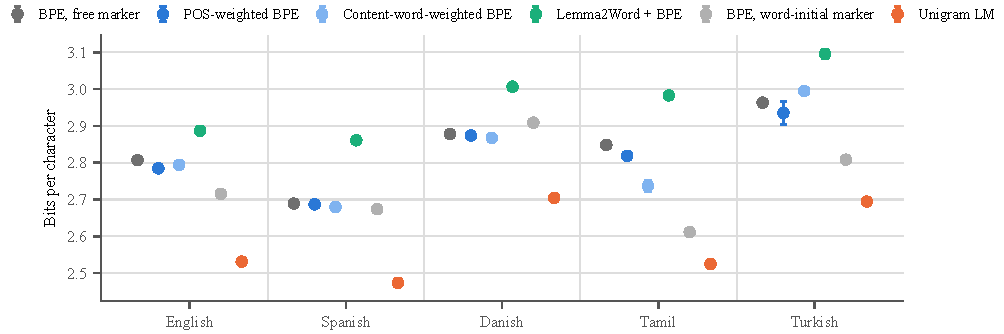
\includegraphics[width=\linewidth]{figures/fig_bpc.pdf}
\caption{Bits per character in the language model trained on the output of the tokenizer. The language model has 7M parameters and is trained for 6 passes over the same text with each tokenizer. Lower scores are better, and we show the mean and one standard deviation for the three tokenizer seeds. The y-axis starts at 2.4 bits to show the differences.}
\label{fig:bpc}
\end{figure}

However, the ordering by bits-per-character does not match the ordering by boundary-F1.
The unigram model has been ranked second by F1 and first by bits-per-character in all languages.
In English it is first with \nBpcUniEnglish{} bits-per-character compared to \nBpcBpeEnglish{} for free-marker BPE.
In Tamil the first place is taken by the unigram model with \nBpcUniTamil{} bits compared to \nBpcBpeTamil{} for free-marker BPE.
Lemma2Word has been ranked first by F1 and last by bits-per-character in all languages.
In English Lemma2Word is ranked last with \nBpcLtwEnglish{} bits-per-character.
The word cutting using stem boundaries before training the subword tokenizer is removing frequent full-word tokens and adding tokens that are too unpredictable for a model of this size to compensate.

Word-initial BPE has been ranked last by F1 in four languages.
In four languages, it has been ranked ahead of free-marker BPE by bits-per-character.
In English it is ranked ahead with \nBpcHfBpeEnglish{} vs.\ \nBpcBpeEnglish.
The tokens crossing word boundaries, which help compactness in free-marker BPE, do not help in prediction.
POS weighting has been changing bits-per-character by less than 0.03 in all the languages, so it seems it is pointing in a positive direction but with a small contribution.
Interestingly, the table shows that for Turkish the seed-to-seed variation in bits-per-character is the highest.
The two ablations with POS weighting give the same result.
Content word weighting has been reducing bits-per-character in Tamil to \nBpcPosContentTamil{} vs.\ \nBpcBpeTamil.
This was also the language where it has been giving the largest improvement in boundary-F1.
On the other hand, in Turkish content-word weighting has been increasing the bits-per-character numbers.

Since all the tokenizers are trained on the same text, the number of passes is the same for all models; they go over the data 6 times.
Since a higher token count therefore leads to more optimizer steps, the unigram model has 8.6\% more optimizer steps than free-marker BPE in English.
To control for the change in optimizer steps, we have trained a model for free-marker BPE in seed 0 with 10\% fewer optimizer steps (5.4 passes over the data) and 10\% more optimizer steps (6.6 passes).
The bits-per-character changes from \nBpcControlBase{} to \nBpcControlLow{} and \nBpcControlHigh{} respectively.
These changes are small compared to the ones between tokenizers, so the step count cannot be used to explain the model ranking.
Since Lemma2Word has a higher number of tokens than free-marker BPE and it has been ranked behind, the reason cannot be the optimizer step count alone.

These results indicate that morphological alignment and the quality of the model do not move together at this scale, which agrees with the conclusions reached about the unigram model by \citet{bostrom2020bpe}.
This also supports the finding that the intrinsic measures for tokenizers are not perfect predictors for downstream tasks~\cite{ali2024tokenizer,schmidt2024tokenization}.
